%% Figure 2 of the manuscript, the simulation framework, as a standalone source.
%% Added 2026-09-23. The decision flow the framework runs on each scenario set is
%% Figure 1 (fig1_framework.tex); this figure shows the three stages of Section 4
%% around it. Same style file conventions as fig1_framework.tex.
%% Build with: python3 build_fig2_simulation.py <output_dir>
\documentclass[border=2pt]{standalone}
\usepackage{amsmath}
\usepackage{amssymb}
\usepackage{txfonts}
\usepackage{tikz}
\usetikzlibrary{arrows.meta,positioning}
\tikzset{
    box/.style={draw=black!70, rounded corners=1.5pt, align=left, inner sep=4pt,
        execute at begin node={\hyphenpenalty=10000\exhyphenpenalty=10000\relax}},
    inbox/.style={box, fill=black!3},
    stage/.style={box, fill=white},
    outbox/.style={box, fill=black!3},
    flow/.style={-{Latex[length=2.2mm,width=1.5mm]}, line width=0.65pt}
}
\begin{document}
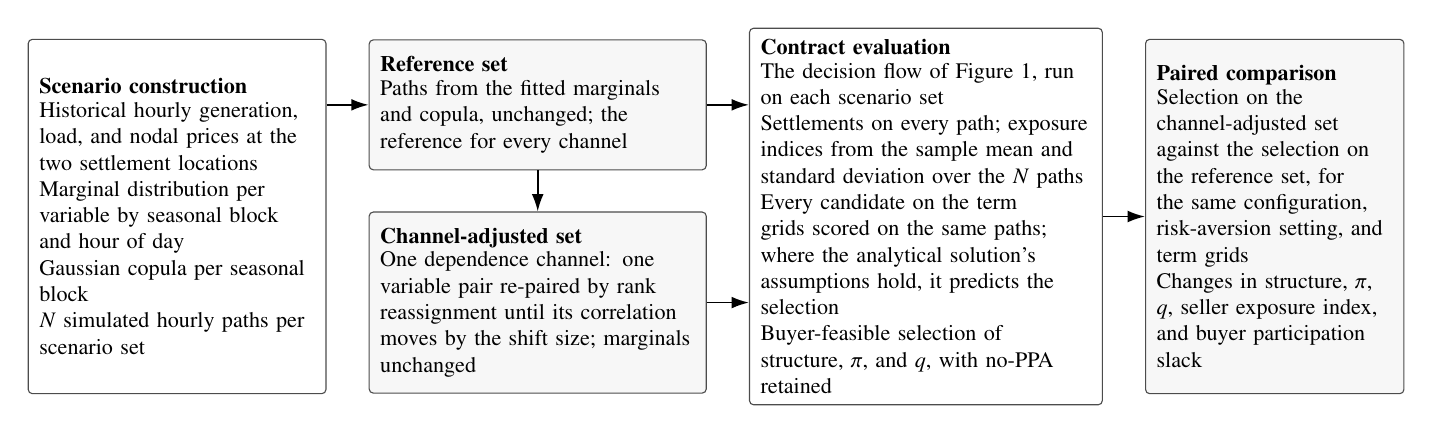
\begin{tikzpicture}[font=\footnotesize]

\node[stage, text width=3.5cm, minimum height=4.5cm] (scen) at (0.0,0) {%
    \textbf{Scenario construction}\\[-1pt]
    Historical hourly generation, load, and nodal prices at the two settlement locations\\
    Marginal distribution per variable by seasonal block and hour of day\\
    Gaussian copula per seasonal block\\
    $N$ simulated hourly paths per scenario set
};
\node[inbox, text width=4.0cm, minimum height=1.65cm, anchor=north] (ref) at (4.58,2.25) {%
    \textbf{Reference set}\\[-1pt]
    Paths from the fitted marginals and copula, unchanged; the reference for every channel
};
\node[inbox, text width=4.0cm, minimum height=2.3cm, anchor=south] (adj) at (4.58,-2.25) {%
    \textbf{Channel-adjusted set}\\[-1pt]
    One dependence channel: one variable pair re-paired by rank reassignment until its correlation moves by the shift size; marginals unchanged
};
\node[stage, text width=4.2cm, minimum height=4.5cm] (eval) at (9.51,0) {%
    \textbf{Contract evaluation}\\[-1pt]
    The decision flow of Figure~1, run on each scenario set\\
    Settlements on every path; exposure indices from the sample mean and standard deviation over the $N$ paths\\
    Every candidate on the term grids scored on the same paths; where the analytical solution's assumptions hold, it predicts the selection\\
    Buyer-feasible selection of structure, $\pi$, and $q$, with no-PPA retained
};
\node[outbox, text width=3.0cm, minimum height=4.5cm] (cmp) at (13.94,0) {%
    \textbf{Paired comparison}\\[-1pt]
    Selection on the channel-adjusted set against the selection on the reference set, for the same configuration, risk-aversion setting, and term grids\\
    Changes in structure, $\pi$, $q$, seller exposure index, and buyer participation slack
};
\draw[flow] (scen.east |- ref.west) -- (ref.west);
\draw[flow] (ref.south) -- (adj.north);
\draw[flow] (ref.east) -- (ref.east -| eval.west);
\draw[flow] (adj.east) -- (adj.east -| eval.west);
\draw[flow] (eval.east) -- (cmp.west);
\end{tikzpicture}
\end{document}
